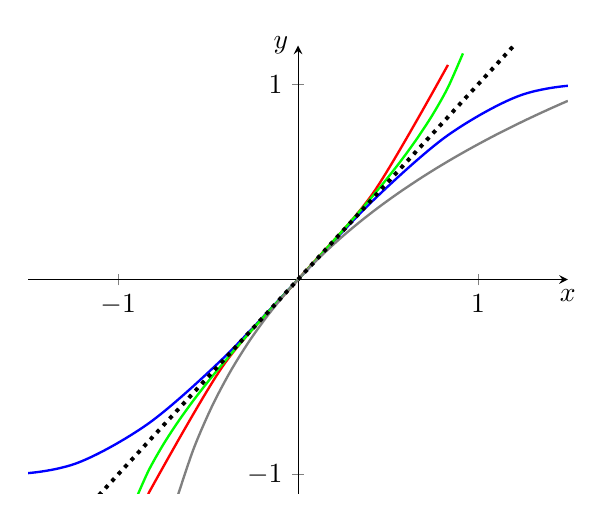
\begin{tikzpicture}[>=stealth][scale = 0.85]
    \begin{axis}[
	axis x line=center,
	axis y line=center,
	xlabel={$x$},
	ylabel={$y$},
	xtick distance=1,
	ytick distance=1,
	xlabel style={below},
	ylabel style={left},
	xmin=-1.5,
	xmax=1.5,
	ymin=-1.1,
	ymax=1.2,
	smooth,
	restrict y to domain=-1.5:1.5,    % <-- added
	]
	\addplot [domain=pi/2:3*pi/2,thick]         {tan(deg(x))};
			\addplot[line width =.03cm,color = blue]  {sin(deg(x))};
			\addplot[line width =.03cm, color = red]  {tan(deg(x))};
			\addplot[line width =.03cm,domain=-1:1,green] {asin(x)/180*pi};
			\addplot[line width =.03cm,color = gray,domain=-1:1.5]  {ln(1+x)};
			\addplot[line width =.05cm, dotted]  {x};
		\end{axis}
\end{tikzpicture}
